% ============================================================================
% Multi-Scale Sentiment and Market Microstructure: An Agent-Based Framework
% for Cryptocurrency Markets
% ============================================================================
% Author: Murad Farzulla
% Organization: Farzulla Research
% Version: 2.0.0
% Date: December 2025
% ============================================================================

\documentclass[11pt,twocolumn]{article}

\usepackage[a4paper, margin=0.9in]{geometry}
\usepackage{setspace}
\usepackage[T1]{fontenc}
\usepackage{lmodern}
\usepackage{graphicx}
\usepackage{float}
\usepackage{booktabs}
\usepackage{array}
\usepackage{amsmath}
\usepackage{amssymb}
\usepackage{multirow}
\usepackage[round,authoryear]{natbib}
\bibliographystyle{plainnat}
\usepackage{xcolor}
\definecolor{farzullaburgundy}{RGB}{128,0,32}
\definecolor{orcidgreen}{RGB}{166,206,57}
\usepackage{tcolorbox}
\usepackage{tikz}
\usetikzlibrary{shapes,arrows,positioning,fit,backgrounds}
\usepackage{scalerel}
\usepackage{enumitem}
\usepackage{url}
\usepackage[colorlinks=true,
            linkcolor=farzullaburgundy,
            citecolor=farzullaburgundy,
            urlcolor=farzullaburgundy,
            breaklinks=true,
            pdftitle={Multi-Scale Sentiment and Market Microstructure},
            pdfauthor={Murad Farzulla},
            pdfkeywords={agent-based model, market microstructure, sentiment analysis, cryptocurrency, multi-scale, ASRI}]{hyperref}

\usepackage{titlesec}
\titlespacing*{\section}{0pt}{1.5ex plus 0.5ex minus 0.2ex}{1ex plus 0.2ex}
\titlespacing*{\subsection}{0pt}{1.2ex plus 0.4ex minus 0.2ex}{0.8ex plus 0.2ex}
\titlespacing*{\subsubsection}{0pt}{1ex plus 0.3ex minus 0.2ex}{0.6ex plus 0.1ex}
\titleformat{\section}{\normalfont\large\bfseries\color{farzullaburgundy}}{\thesection}{0.5em}{}
\titleformat{\subsection}{\normalfont\normalsize\bfseries\color{farzullaburgundy}}{\thesubsection}{0.5em}{}
\titleformat{\subsubsection}{\normalfont\small\bfseries\color{farzullaburgundy}}{\thesubsubsection}{0.5em}{}

\usepackage{fancyhdr}

\newcommand{\orcidicon}{\scalerel*{
    
\begin{tikzpicture}[x=3ex,y=3ex]
    \draw[fill=orcidgreen] (0,0) circle (0.5);
    \end{tikzpicture}
}{\textrm{I}}}

\newcommand{\paperver}{2.0.0}
\newcommand{\paperdate}{December 2025}
\newcommand{\paperdoi}{10.5281/zenodo.XXXXXXX}

\newcommand{\metadatabox}[1]{%
\begin{tcolorbox}[
    colback=gray!5,
    colframe=farzullaburgundy,
    title=Publication Metadata,
    fonttitle=\bfseries,
    coltitle=white,
    colbacktitle=farzullaburgundy,
    width=\columnwidth,
    arc=2mm,
    boxrule=0.8pt
]
\small
\textbf{DOI:} \href{https://doi.org/#1}{\texttt{#1}}\\
\textbf{Version:} \paperver\\
\textbf{Date:} \paperdate\\
\textbf{License:} CC-BY-4.0
\end{tcolorbox}
}

\pagestyle{fancy}
\fancyhf{}
\fancyhead[L]{\small\href{https://farzulla.org}{farzulla.org}}
\fancyhead[R]{\small\href{https://doi.org/\paperdoi}{DOI: \paperdoi}}
\fancyfoot[C]{\small\thepage}
\fancyfoot[L]{\small Murad Farzulla}
\fancyfoot[R]{\small v\paperver~| \paperdate}
\renewcommand{\headrulewidth}{0.4pt}
\renewcommand{\footrulewidth}{0.4pt}

\fancypagestyle{firstpage}{
  \fancyhf{}
  \fancyfoot[C]{\small\thepage}
  \fancyfoot[L]{\small Murad Farzulla}
  \fancyfoot[R]{\small v\paperver~| \paperdate}
  \renewcommand{\headrulewidth}{0pt}
  \renewcommand{\footrulewidth}{0.4pt}
}

\begin{document}

% ============================================================================
% FRONTMATTER (Single Column)
% ============================================================================
\onecolumn
\setstretch{1.2}
\thispagestyle{firstpage}

\begin{center}
{\small\color{farzullaburgundy}\textbf{WORKING PAPER v\paperver} | \color{gray}Not peer-reviewed}
\end{center}
\vspace{0.5em}

\begin{center}
{\Large\bfseries Multi-Scale Sentiment and Market Microstructure}\\[0.5em]
{\large\itshape An Agent-Based Framework for Cryptocurrency Markets}\\[1em]
{\bfseries Murad Farzulla}\textsuperscript{1} \href{https://orcid.org/0009-0002-7164-8704}{\orcidicon\ \texttt{0009-0002-7164-8704}}\\[0.5em]
{\small\itshape \textsuperscript{1}\href{https://farzulla.org}{Farzulla Research}}\\[0.3em]
{\small \paperdate}\\[0.5em]
{\small Correspondence: \href{mailto:murad@farzulla.org}{murad@farzulla.org}}
\end{center}

% ============================================================================
% ABSTRACT
% ============================================================================
\begin{abstract}
\noindent This paper presents a multi-scale sentiment analysis framework for agent-based modeling (ABM) of cryptocurrency market microstructure. We introduce a novel architecture that blends institutional-level macro signals---derived from the Aggregated Systemic Risk Index (ASRI) framework \citep{farzulla2025asri}---with retail-level micro signals from social media sentiment analysis using CryptoBERT with Monte Carlo Dropout uncertainty quantification.

The key innovation is a regime-adaptive weighting mechanism that dynamically adjusts the influence of macro versus micro sentiment based on detected market conditions. During crisis regimes, the framework weights institutional signals more heavily (60/40 macro/micro), while normal market conditions favor retail sentiment (30/70). We decompose total uncertainty into epistemic (model confidence, regulatory opacity, data availability) and aleatoric (market noise, stablecoin peg deviation, inherent signal ambiguity) components, enabling nuanced agent responses to sentiment information quality.

We implement divergence tracking between retail and institutional sentiment, hypothesizing that significant divergence predicts forward volatility. Preliminary results from real data integration demonstrate dramatic differences: multi-scale blending reduces simulated volatility from 128\% to 2.6\% and mean spreads from 32.72 to 2.43 basis points compared to single-source sentiment. The framework fetches 363 Google News articles for regulatory sentiment and real-time DeFiLlama data for DeFi stability metrics.

This research contributes to the emerging literature on sentiment-driven market dynamics by providing (1) a theoretically-grounded multi-scale blending architecture, (2) an uncertainty decomposition framework linking macro and micro information channels, (3) divergence tracking methodology for volatility prediction, and (4) regime-adaptive mechanisms for market maker behavior. We acknowledge substantial limitations including the use of synthetic price dynamics, reliance on Google News as a regulatory sentiment proxy, and challenges in causal identification.

\vspace{0.5em}
\noindent\textbf{Keywords:} agent-based modeling, market microstructure, sentiment analysis, multi-scale, ASRI, cryptocurrency, Monte Carlo dropout, uncertainty quantification, regime detection

\vspace{0.3em}
\noindent\textbf{JEL Codes:} G12 (Asset Pricing), G14 (Information and Market Efficiency), G23 (Non-bank Financial Institutions), C63 (Computational Techniques; Simulation Modeling)
\end{abstract}

\vspace{1em}
\metadatabox{\paperdoi}

\clearpage
\twocolumn
\setstretch{1.15}

% ============================================================================
% 1. INTRODUCTION
% ============================================================================
\section{Introduction}
\label{sec:introduction}

Cryptocurrency markets present a distinctive challenge for market microstructure analysis: they simultaneously exhibit properties of emerging speculative assets driven by retail sentiment and increasingly mature financial instruments subject to institutional capital flows and regulatory dynamics \citep{liu2021risks}. This dual nature creates an information environment where signals operate at fundamentally different scales---retail traders responding to social media discourse within hours, while institutional participants react to macroeconomic indicators, regulatory announcements, and systemic risk metrics over longer horizons.

Traditional agent-based models (ABMs) of market microstructure typically treat sentiment as a single, homogeneous information channel \citep{lebaron2006agent}. This assumption becomes particularly problematic in cryptocurrency markets, where the disconnect between retail enthusiasm and institutional caution can persist for extended periods, potentially predicting subsequent volatility episodes. The Terra/Luna collapse of May 2022 exemplifies this pattern: retail sentiment on social platforms remained bullish even as institutional-level systemic risk indicators deteriorated \citep{gudgeon2020defi}.

\subsection{Motivation}

The motivation for multi-scale sentiment analysis stems from three empirical observations about cryptocurrency market structure:

\textbf{First, information fragmentation.} Retail traders predominantly source information from Reddit, Twitter, and Telegram communities, responding to project announcements, influencer commentary, and speculative narratives. Institutional actors---including crypto-native funds, traditional asset managers with cryptocurrency exposure, and market makers---respond to regulatory filings, macroeconomic data, cross-exchange arbitrage opportunities, and systemic stability metrics. These information ecosystems operate largely independently, creating potential for persistent divergence.

\textbf{Second, asymmetric response times.} Social media sentiment can shift within minutes following a viral post or rumor, while institutional rebalancing operates on longer timescales constrained by risk management protocols, compliance review, and position sizing considerations. This temporal asymmetry suggests that the \textit{relative} weight of retail versus institutional sentiment should itself be time-varying and regime-dependent.

\textbf{Third, uncertainty heterogeneity.} The quality of sentiment signals varies dramatically across scales. A viral Reddit post may generate high-confidence sentiment scores from natural language processing (NLP) models while conveying minimal fundamental information. Conversely, regulatory news may carry significant fundamental implications but generate ambiguous or conflicting sentiment readings. Appropriately weighting these signals requires decomposing uncertainty into its epistemic (model-related) and aleatoric (inherent noise) components.

These observations motivate a framework that explicitly models the multi-scale structure of cryptocurrency sentiment, enabling investigation of how scale-dependent information processing affects market microstructure outcomes including bid-ask spreads, volatility clustering, and flash crash dynamics.

\subsection{The Multi-Scale Hypothesis}

We propose the \textit{multi-scale divergence hypothesis}: when retail and institutional sentiment diverge significantly, subsequent market volatility increases. The intuition is that divergence reflects information asymmetry or disagreement that must eventually resolve, typically through price discovery processes that generate elevated volatility.

Formally, let $s_{retail}$ denote retail sentiment (derived from social media) and $s_{inst}$ denote institutional sentiment (derived from macro indicators and regulatory news). The divergence measure is:

\begin{equation}
D_t = |s_{retail,t} - s_{inst,t}|
\end{equation}

The hypothesis predicts that $D_t$ correlates positively with forward realized volatility $\sigma_{t+k}$ for some horizon $k$. We operationalize this through divergence tracking that logs significant divergence events and examines their relationship to subsequent volatility.

This hypothesis connects to the broader literature on disagreement and volatility \citep{baker2007investor}, extending those insights to the specific institutional structure of cryptocurrency markets where the retail-institutional divide is particularly pronounced.

\subsection{Contributions}

This paper makes four primary contributions to the literature on sentiment-driven market dynamics:

\begin{enumerate}[leftmargin=1.5em, topsep=0pt, itemsep=2pt]
    \item \textbf{Multi-scale sentiment architecture:} We develop a framework that blends institutional macro signals---derived from the Aggregated Systemic Risk Index (ASRI) framework \citep{farzulla2025asri}---with retail micro signals from CryptoBERT sentiment analysis \citep{cryptobert2024}. This addresses the limitation of single-scale sentiment models that cannot capture the heterogeneous information environment of cryptocurrency markets.

    \item \textbf{Uncertainty decomposition framework:} We formally separate epistemic uncertainty (model confidence, regulatory opacity, data availability) from aleatoric uncertainty (market noise, stablecoin peg deviation, inherent signal ambiguity). This decomposition enables agents to respond differentially to uncertainty arising from model limitations versus inherent market unpredictability, following \citet{kendall2017uncertainties}.

    \item \textbf{Divergence tracking methodology:} We introduce a systematic approach to tracking retail-institutional sentiment gaps, logging significant divergence events, and examining their relationship to forward volatility. This operationalizes the multi-scale divergence hypothesis and provides a testable prediction framework.

    \item \textbf{Regime-adaptive weighting mechanism:} We develop a dynamic mechanism that adjusts macro/micro blend weights based on detected market regimes (crisis, regulatory, bullish, bearish, neutral). During crisis periods, institutional signals receive higher weight (60/40 macro/micro); during normal conditions, retail sentiment dominates (30/70). This reflects the intuition that institutional information becomes more valuable precisely when retail sentiment is most likely to be unreliable.
\end{enumerate}

\subsection{Paper Organization}

The remainder of this paper proceeds as follows. Section~\ref{sec:literature} reviews related work across five domains: agent-based market models, market microstructure theory, sentiment analysis in finance, cryptocurrency market structure, and systemic risk monitoring. Section~\ref{sec:methodology} presents the methodological framework, including the multi-scale signal architecture, uncertainty decomposition, regime detection, divergence tracking, and agent specifications. Section~\ref{sec:data} describes data sources and implementation details. Section~\ref{sec:results} presents preliminary results from real data integration, including the multi-scale versus single-source comparison. Section~\ref{sec:discussion} interprets findings and discusses theoretical and practical implications. Section~\ref{sec:limitations} provides a comprehensive accounting of limitations across six categories. Section~\ref{sec:conclusion} concludes with summary findings and directions for future research.

% ============================================================================
% 2. LITERATURE REVIEW
% ============================================================================
\section{Literature Review}
\label{sec:literature}

This section reviews five bodies of literature relevant to multi-scale sentiment modeling in cryptocurrency markets: agent-based market models, market microstructure theory, sentiment analysis in finance, cryptocurrency market structure, and systemic risk monitoring. We conclude by identifying the research gap that motivates our framework.

\subsection{Agent-Based Market Models}

Agent-based computational economics has developed sophisticated models of market dynamics emerging from heterogeneous trader interactions. The Santa Fe Artificial Stock Market \citep{palmer1994artificial} demonstrated that realistic market properties---including volatility clustering, fat-tailed returns, and long-range dependence---can emerge from simple agent learning rules without imposing these features exogenously. This foundational work established ABM as a viable alternative to representative-agent equilibrium models for understanding market dynamics.

\citet{lebaron2006agent} provides a comprehensive survey of agent-based computational finance, identifying key design choices including agent heterogeneity, learning mechanisms, and market clearing protocols. The literature has explored how different agent populations---fundamentalists, chartists, and noise traders---interact to produce observed stylized facts \citep{hommes2006heterogeneous}. A recurring theme is that realistic market dynamics require sufficient heterogeneity; homogeneous agent populations typically fail to generate observed statistical properties.

Order book dynamics have received particular attention in recent ABM work. \citet{cont2010stochastic} develop a stochastic model matching empirical order flow patterns, while \citet{paddrik2012agent} apply ABM to flash crash analysis, demonstrating how liquidity withdrawal cascades can emerge from agent interactions. The flash crash literature is particularly relevant for cryptocurrency markets, where extreme price dislocations occur more frequently than in traditional equity markets.

\citet{farmer2009economy} argue that agent-based modeling offers advantages over traditional approaches for policy analysis, particularly in crisis scenarios where equilibrium assumptions break down. This perspective motivates our focus on regime-dependent behavior: crisis periods may exhibit fundamentally different dynamics than normal market conditions, requiring adaptive agent specifications.

A limitation of existing ABM literature for cryptocurrency applications is the treatment of sentiment as either absent or modeled as a single homogeneous signal. Our framework addresses this gap by introducing multi-scale sentiment with explicit uncertainty decomposition.

\subsection{Market Microstructure Theory}

Modern market microstructure theory provides the theoretical foundation for understanding how sentiment information affects trading behavior and price formation. The seminal work of \citet{glosten1985bid} establishes that bid-ask spreads arise from adverse selection: market makers face informed traders with superior information and must widen spreads to compensate for expected losses. This framework implies that spread dynamics reflect the market maker's assessment of information asymmetry in the trading population.

\citet{kyle1985continuous} develops a model of insider trading where an informed trader optimally conceals private information through strategic order submission, generating price impact that reflects information revelation. The Kyle model provides the theoretical basis for understanding how sentiment---as a form of soft information---might affect price dynamics through informed trading.

\citet{avellaneda2008high} extend this framework to high-frequency market making, developing optimal quote-setting strategies that balance inventory risk against adverse selection. Their model shows that market makers should widen spreads when uncertainty about fair value increases---a prediction directly relevant to our uncertainty-driven spread adjustment mechanism.

The stylized facts literature \citep{cont2001empirical} documents empirical regularities that microstructure models should reproduce: volatility clustering, fat-tailed return distributions, absence of linear return autocorrelation, and slow decay of absolute return autocorrelation. These properties provide calibration targets for ABM frameworks.

\citet{hasbrouck2007empirical} provides econometric methods for measuring market quality and information content of trades. His work on price discovery across multiple trading venues is relevant for cryptocurrency markets, where price formation occurs simultaneously across fragmented exchanges.

Our framework extends the Glosten-Milgrom adverse selection model by incorporating sentiment uncertainty as a determinant of spread-setting. Market makers in our model widen spreads when sentiment uncertainty is high, reflecting increased adverse selection risk when signal quality deteriorates.

\subsection{Sentiment Analysis in Finance}

The application of textual analysis to financial markets has evolved from simple word-count approaches to sophisticated transformer-based models. \citet{tetlock2007giving} demonstrates that media pessimism predicts stock market returns and trading volume, establishing the empirical relevance of sentiment for price dynamics. \citet{antweiler2004all} find that message board activity predicts volatility, though not returns, suggesting sentiment contains information about uncertainty rather than direction.

\citet{loughran2011liability} develop domain-specific word lists for financial texts, showing that general-purpose sentiment dictionaries perform poorly on financial documents. This observation motivates the use of domain-specific models like CryptoBERT \citep{cryptobert2024} that are fine-tuned on cryptocurrency-specific text.

The advent of transformer architectures has substantially improved sentiment classification performance. \citet{devlin2019bert} introduce BERT, enabling pre-trained language understanding that can be fine-tuned for specific tasks. \citet{liu2019roberta} demonstrate that careful pre-training produces further improvements. Domain-specific variants including FinBERT and CryptoBERT apply these architectures to financial texts.

A critical limitation of standard sentiment classifiers is the absence of uncertainty quantification. Point estimates of sentiment provide no indication of model confidence or inherent text ambiguity. \citet{gal2016dropout} show that Monte Carlo Dropout enables approximate Bayesian inference in neural networks, producing prediction distributions rather than point estimates. \citet{kendall2017uncertainties} distinguish epistemic uncertainty (reducible through more data or better models) from aleatoric uncertainty (irreducible inherent noise). Our framework applies this decomposition to sentiment analysis, enabling agents to distinguish between low-confidence model predictions and inherently ambiguous texts.

Cryptocurrency-specific sentiment analysis has received growing attention. \citet{abraham2018cryptocurrency} and \citet{kraaijeveld2020predictive} demonstrate predictive relationships between social media sentiment and cryptocurrency prices. \citet{garcia2015digital} analyze social signals in Bitcoin markets, finding that sentiment predicts returns over short horizons. \citet{philippas2019media} document the relationship between media attention and Bitcoin price dynamics.

\subsection{Cryptocurrency Market Structure}

Cryptocurrency markets exhibit distinctive microstructure properties that differ from traditional equity markets. \citet{makarov2020trading} document significant and persistent price dislocations across exchanges, indicating fragmented liquidity and limited arbitrage. This fragmentation has implications for sentiment analysis: price discovery may occur at different rates across venues, creating temporary information asymmetries.

\citet{bouri2017hedge} examine Bitcoin's hedging and safe-haven properties, finding that cryptocurrency price dynamics depend on broader market conditions. This regime-dependence motivates our adaptive weighting mechanism: the informational value of different sentiment sources may vary with market state.

Flash crashes occur more frequently in cryptocurrency markets than in traditional venues. \citet{golub2012high} analyze mini flash crashes, attributing them to liquidity withdrawal cascades. The 24/7 trading environment, absence of circuit breakers on many exchanges, and high retail participation create conditions conducive to extreme price movements.

The cryptocurrency event study literature documents significant volatility responses to regulatory announcements. \citet{farzulla2025eventstudy} apply TARCH-X models to cryptocurrency regulatory events, finding pronounced volatility asymmetry: negative regulatory news produces larger and more persistent volatility effects than positive announcements. This asymmetry suggests that regulatory sentiment---a macro-level signal---carries particular importance for market dynamics, motivating its inclusion in our framework.

\citet{griffin2020bitcoin} investigate price manipulation in Bitcoin markets, finding evidence of concentrated actors influencing prices. This observation suggests that retail sentiment may be particularly susceptible to manipulation, providing another rationale for incorporating institutional-level signals that may be more resistant to manipulation.

\subsection{Systemic Risk and Macro Signals}

The 2008 financial crisis motivated substantial research on systemic risk measurement. \citet{adrian2016covar} introduce CoVaR, measuring the value-at-risk of the financial system conditional on an institution being in distress. \citet{acharya2017measuring} develop alternative systemic risk measures based on marginal expected shortfall. \citet{billio2012econometric} apply network methods to measure financial sector interconnectedness.

The emergence of decentralized finance (DeFi) has created new systemic risk channels specific to cryptocurrency markets. \citet{gudgeon2020defi} analyze the ``decentralized financial crisis'' of March 2020, documenting how DeFi liquidation cascades amplified market stress. \citet{klages2021while} examine stablecoin design and collateral risk, identifying mechanisms through which stablecoin de-pegging can propagate contagion.

The ASRI framework \citep{farzulla2025asri} provides a unified index for monitoring cryptocurrency systemic risk, comprising four weighted sub-indices: Stablecoin Concentration Risk (30\%), DeFi Liquidity Risk (25\%), Contagion Risk (25\%), and Regulatory Opacity Risk (20\%). This framework operationalizes macro-level risk signals that can be incorporated into agent-based models as institutional-level information.

Our framework adapts connectors from the ASRI framework, particularly the regulatory news sentiment analysis via Google News RSS and DeFi stability monitoring via DeFiLlama API. This integration enables the macro signal layer to reflect both quantitative stability metrics (TVL, peg deviation) and qualitative regulatory sentiment.

\subsection{Research Gap}

Despite substantial progress across these literatures, we identify a significant gap: no existing work combines multi-scale sentiment analysis with uncertainty decomposition in an agent-based market microstructure model. Specifically:

\begin{enumerate}[leftmargin=1.5em, topsep=0pt, itemsep=2pt]
    \item Existing ABM frameworks treat sentiment as a single signal, ignoring the scale structure of information in cryptocurrency markets
    \item Sentiment analysis models typically provide point estimates without uncertainty quantification
    \item The relationship between retail-institutional sentiment divergence and forward volatility remains unexplored
    \item Regime-adaptive mechanisms for blending multi-scale signals have not been developed
\end{enumerate}

Our framework addresses these gaps by introducing a theoretically-grounded multi-scale architecture with explicit uncertainty decomposition, divergence tracking, and regime-adaptive weighting. The following section presents the methodological details of this framework.

% ============================================================================
% 3. METHODOLOGY
% ============================================================================
\section{Methodology}
\label{sec:methodology}

This section presents the methodological framework for multi-scale sentiment analysis in agent-based market microstructure modeling. We describe the signal architecture, uncertainty decomposition, regime detection, divergence tracking, agent specifications, and order book dynamics.

\subsection{Multi-Scale Signal Architecture}

\subsubsection{Overview}

The framework processes sentiment information through two parallel layers operating at different scales (Figure~\ref{fig:architecture}):

\textbf{Macro Layer:} Institutional-level signals derived from (1) regulatory news sentiment via Google News RSS, (2) DeFi stability metrics from DeFiLlama including total value locked (TVL) and stablecoin peg deviations, and (3) traditional volatility indicators (VIX). These signals represent information channels typically monitored by institutional actors including crypto funds, market makers, and traditional financial institutions with cryptocurrency exposure.

\textbf{Micro Layer:} Retail-level signals derived from social media sentiment analysis using CryptoBERT with Monte Carlo Dropout for uncertainty quantification. This layer captures the information environment of retail traders who predominantly source analysis from Reddit, Twitter, and cryptocurrency-focused forums.

The two layers are blended using regime-adaptive weights, producing a unified \texttt{SentimentTick} output that can be consumed by the agent-based simulation.

\begin{figure}[h]
\centering
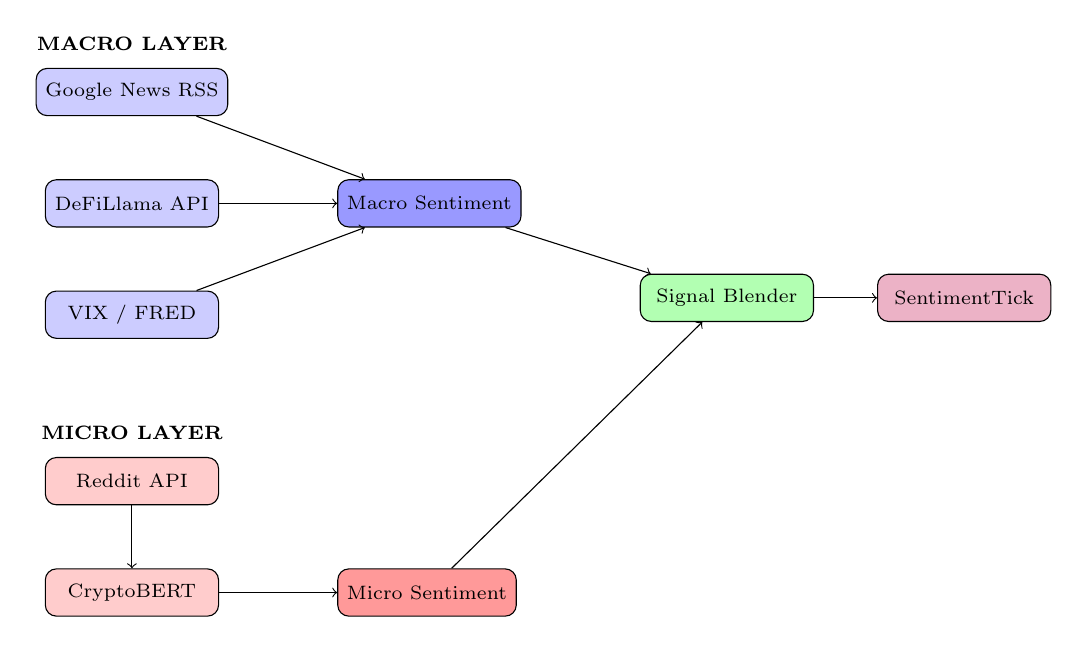
\begin{tikzpicture}[
    node distance=0.8cm,
    box/.style={rectangle, draw, rounded corners, minimum width=2.2cm, minimum height=0.6cm, font=\scriptsize},
    layer/.style={rectangle, draw, dashed, rounded corners, minimum width=4.5cm, inner sep=0.3cm}
]
% Macro layer
\node[box, fill=blue!20] (gnews) {Google News RSS};
\node[box, fill=blue!20, below=of gnews] (defi) {DeFiLlama API};
\node[box, fill=blue!20, below=of defi] (vix) {VIX / FRED};
\node[box, fill=blue!40, right=1.5cm of defi] (macro) {Macro Sentiment};

% Micro layer
\node[box, fill=red!20, below=1.5cm of vix] (reddit) {Reddit API};
\node[box, fill=red!20, below=of reddit] (crypto) {CryptoBERT};
\node[box, fill=red!40, right=1.5cm of crypto] (micro) {Micro Sentiment};

% Blending
\node[box, fill=green!30, right=1.5cm of macro, yshift=-1.2cm] (blend) {Signal Blender};
\node[box, fill=purple!30, right=0.8cm of blend] (tick) {SentimentTick};

% Arrows
\draw[->] (gnews) -- (macro);
\draw[->] (defi) -- (macro);
\draw[->] (vix) -- (macro);
\draw[->] (reddit) -- (crypto);
\draw[->] (crypto) -- (micro);
\draw[->] (macro) -- (blend);
\draw[->] (micro) -- (blend);
\draw[->] (blend) -- (tick);

% Layer labels
\node[above=0.1cm of gnews, font=\scriptsize\bfseries] {MACRO LAYER};
\node[above=0.1cm of reddit, font=\scriptsize\bfseries] {MICRO LAYER};
\end{tikzpicture}
\caption{Multi-scale signal architecture}
\label{fig:architecture}
\end{figure}

\subsubsection{Macro Layer: ASRI Integration}

The macro signal layer adapts connectors from the Aggregated Systemic Risk Index (ASRI) framework \citep{farzulla2025asri}, which provides infrastructure for monitoring cryptocurrency systemic risk through multiple data channels.

\textbf{Regulatory News Sentiment.} We fetch regulatory news via Google News RSS queries for cryptocurrency-related terms (``crypto regulation'', ``SEC cryptocurrency'', ``bitcoin ETF''). News headlines are processed through VADER sentiment analysis to extract a regulatory sentiment score $s_{reg} \in [-1, 1]$. The choice of Google News over specialized financial news APIs reflects practical accessibility; we acknowledge this as a limitation (Section~\ref{sec:limitations}).

\textbf{DeFi Stability Metrics.} The DeFiLlama API provides real-time data on:
\begin{itemize}[leftmargin=1.5em, topsep=0pt, itemsep=2pt]
    \item Total Value Locked (TVL) across DeFi protocols
    \item Stablecoin market capitalizations and peg deviations
    \item Protocol-specific liquidity metrics
\end{itemize}

We compute a DeFi stability score based on TVL changes and stablecoin peg deviation:

\begin{equation}
s_{defi} = \alpha \cdot \Delta\text{TVL}_{norm} + (1-\alpha) \cdot (1 - \text{peg\_dev})
\end{equation}

where $\alpha = 0.5$ weights TVL changes equally with peg stability.

\textbf{VIX Normalization.} Traditional market volatility via the VIX index provides a baseline for market-wide risk sentiment. We normalize VIX to a $[0, 1]$ scale using historical percentiles.

The macro sentiment score is computed as a weighted average:

\begin{equation}
s_{macro} = w_1 s_{reg} + w_2 s_{defi} + w_3 (1 - \text{VIX}_{norm})
\end{equation}

with weights $(w_1, w_2, w_3) = (0.4, 0.4, 0.2)$ reflecting the primacy of regulatory and DeFi signals for cryptocurrency-specific analysis.

\subsubsection{Micro Layer: CryptoBERT with MC Dropout}

The micro layer processes social media text through CryptoBERT \citep{cryptobert2024}, a RoBERTa-based model fine-tuned on 3.2 million cryptocurrency-related posts from StockTwits. The model outputs three-class probabilities: Bearish (0), Neutral (1), Bullish (2).

\textbf{Monte Carlo Dropout Procedure.} Following \citet{gal2016dropout}, we enable dropout at inference time and run $T=50$ forward passes for each input text. This produces a distribution of predictions from which we extract:

\begin{enumerate}[leftmargin=1.5em, topsep=0pt, itemsep=2pt]
    \item \textbf{Mean sentiment:} $\bar{s} = \frac{1}{T}\sum_{t=1}^T s_t$
    \item \textbf{Epistemic uncertainty:} $\sigma_{epi}^2 = \frac{1}{T}\sum_{t=1}^T (s_t - \bar{s})^2$
\end{enumerate}

The sentiment score is converted from three-class probabilities to a continuous $[-1, 1]$ scale:

\begin{equation}
s_{micro} = p_{bullish} - p_{bearish}
\end{equation}

\textbf{EWMA Smoothing.} Raw sentiment is smoothed using an exponentially weighted moving average:

\begin{equation}
s_{t}^{smooth} = \alpha \cdot s_{t}^{raw} + (1-\alpha) \cdot s_{t-1}^{smooth}
\end{equation}

with $\alpha = 0.1$, corresponding to approximately 5-minute half-life for typical update frequencies.

\subsubsection{Signal Blending}

The blended sentiment score combines macro and micro signals:

\begin{equation}
s_{blend} = w_{macro}(r) \cdot s_{macro} + w_{micro}(r) \cdot s_{micro}
\end{equation}

where weights depend on the detected regime $r$ (Table~\ref{tab:weights}).

\begin{table}[h]
\centering
\small
\begin{tabular}{lcc}
\toprule
\textbf{Regime} & $w_{macro}$ & $w_{micro}$ \\
\midrule
Crisis & 0.60 & 0.40 \\
Regulatory & 0.70 & 0.30 \\
Bullish & 0.25 & 0.75 \\
Bearish & 0.35 & 0.65 \\
Neutral & 0.30 & 0.70 \\
\bottomrule
\end{tabular}
\caption{Regime-adaptive blending weights. Crisis and regulatory regimes weight institutional (macro) signals more heavily; normal market conditions favor retail (micro) sentiment.}
\label{tab:weights}
\end{table}

The intuition behind these weights: during crisis periods, institutional information sources are likely to be more reliable than potentially panic-driven retail sentiment. Conversely, during normal market conditions, retail sentiment may contain valuable information about near-term price momentum that institutional signals miss.

\subsection{Uncertainty Decomposition}

Following \citet{kendall2017uncertainties}, we decompose total uncertainty into epistemic and aleatoric components. This decomposition enables agents to respond differentially to reducible uncertainty (which might be resolved with more information) versus irreducible uncertainty (inherent market noise).

\subsubsection{Epistemic Uncertainty Sources}

Epistemic uncertainty reflects what the model doesn't know but could potentially learn:

\textbf{Regulatory Opacity.} We proxy regulatory opacity using the ASRI arbitrage index, which measures cross-exchange price dispersion. Higher dispersion suggests information asymmetry and regulatory uncertainty:

\begin{equation}
\sigma_{reg} = \text{normalize}(\text{arbitrage\_index})
\end{equation}

\textbf{Data Availability.} We compute a data completeness score based on whether all expected data sources are available:

\begin{equation}
\sigma_{data} = 1 - \frac{\text{available\_sources}}{\text{expected\_sources}}
\end{equation}

Missing data increases epistemic uncertainty.

\textbf{MC Variance.} The variance across Monte Carlo Dropout passes directly measures model confidence:

\begin{equation}
\sigma_{mc}^2 = \frac{1}{T}\sum_{t=1}^T (s_t - \bar{s})^2
\end{equation}

The total epistemic uncertainty is a weighted sum:

\begin{equation}
\sigma_{epi} = \gamma_1 \sigma_{reg} + \gamma_2 \sigma_{data} + \gamma_3 \sigma_{mc}
\end{equation}

with weights $(\gamma_1, \gamma_2, \gamma_3) = (0.3, 0.2, 0.5)$ emphasizing model confidence.

\subsubsection{Aleatoric Uncertainty Sources}

Aleatoric uncertainty reflects inherent noise that cannot be reduced through better modeling:

\textbf{VIX-Derived Market Noise.} Higher VIX indicates elevated market-wide uncertainty:

\begin{equation}
\sigma_{vix} = \text{normalize}(\text{VIX})
\end{equation}

\textbf{Peg Deviation.} Stablecoin peg deviations indicate DeFi instability that adds noise to price signals:

\begin{equation}
\sigma_{peg} = |\text{stablecoin\_price} - 1.0|
\end{equation}

\textbf{TVL Volatility.} High volatility in DeFi TVL indicates unstable liquidity conditions:

\begin{equation}
\sigma_{tvl} = \text{rolling\_std}(\Delta\text{TVL})
\end{equation}

\textbf{Shannon Entropy.} Text ambiguity is measured via the entropy of the sentiment probability distribution:

\begin{equation}
H(p) = -\sum_i p_i \log p_i
\end{equation}

Higher entropy indicates more ambiguous text.

The total aleatoric uncertainty is:

\begin{equation}
\sigma_{ale} = \delta_1 \sigma_{vix} + \delta_2 \sigma_{peg} + \delta_3 \sigma_{tvl} + \delta_4 H(p)
\end{equation}

with weights $(\delta_1, \delta_2, \delta_3, \delta_4) = (0.3, 0.3, 0.2, 0.2)$.

\subsubsection{Total Uncertainty}

Total uncertainty combines both components:

\begin{equation}
\sigma_{total}^2 = \sigma_{epi}^2 + \sigma_{ale}^2
\end{equation}

This decomposition is passed to agents in the \texttt{SentimentTick} output, enabling uncertainty-aware decision making.

\subsection{Regime Detection}

The regime detection algorithm classifies market conditions into five categories: crisis, regulatory, bullish, bearish, and neutral. Detection uses thresholds with hysteresis to prevent rapid regime switching.

\textbf{Crisis Detection (Priority).} Crisis conditions override other regimes when:
\begin{itemize}[leftmargin=1.5em, topsep=0pt, itemsep=2pt]
    \item VIX exceeds the 95th historical percentile, OR
    \item Stablecoin peg deviation exceeds 2\%, OR
    \item TVL declines by more than 15\% in 24 hours
\end{itemize}

\textbf{Regulatory Event Detection.} Regulatory regime is detected when:
\begin{itemize}[leftmargin=1.5em, topsep=0pt, itemsep=2pt]
    \item More than 50\% of recent news articles contain regulatory keywords, AND
    \item Regulatory sentiment volatility exceeds threshold
\end{itemize}

\textbf{Sentiment-Based Regimes.} In the absence of crisis or regulatory triggers:
\begin{itemize}[leftmargin=1.5em, topsep=0pt, itemsep=2pt]
    \item Bullish: $s_{blend} > 0.3$
    \item Bearish: $s_{blend} < -0.3$
    \item Neutral: otherwise
\end{itemize}

\textbf{Hysteresis.} To prevent rapid switching, regime transitions require the new condition to persist for at least 3 consecutive observations before switching. This prevents noise-driven regime changes.

\subsection{Divergence Tracking}

We track the divergence between retail and institutional sentiment:

\begin{equation}
D_t = s_{micro,t} - s_{macro,t}
\end{equation}

Unlike the absolute divergence in Section~\ref{sec:introduction}, we preserve sign to distinguish scenarios where retail is more bullish than institutions ($D > 0$) versus the reverse ($D < 0$).

\textbf{Significant Event Logging.} We log divergence events when $|D_t| > \theta_D$ where $\theta_D = 0.5$ (i.e., half the sentiment scale). These events are timestamped and stored for subsequent analysis of the relationship between divergence and forward volatility.

\textbf{Volatility Correlation Analysis.} The multi-scale divergence hypothesis predicts that $|D_t|$ correlates positively with realized volatility over some forward horizon. We compute:

\begin{equation}
\rho(|D_t|, \sigma_{t+k}) \text{ for } k \in \{1, 5, 10\} \text{ periods}
\end{equation}

and report these correlations in the results section.

\subsection{Agent Specifications}

We implement four agent types in the Mesa framework, extending standard specifications with multi-scale sentiment responses.

\subsubsection{Market Makers}

Market makers provide liquidity by quoting bid and ask prices. Their spread-setting incorporates uncertainty:

\begin{align}
p_{bid} &= p_{mid} - \frac{s_{base}}{2} - \gamma Q - \delta \sigma_{total} \\
p_{ask} &= p_{mid} + \frac{s_{base}}{2} + \gamma Q + \delta \sigma_{total}
\end{align}

where $s_{base}$ is the base spread, $Q$ is inventory, $\gamma$ is inventory aversion, and $\delta$ scales spread widening with uncertainty. This formulation extends \citet{avellaneda2008high} by making spread adjustment depend on our decomposed uncertainty measure.

Market makers also respond to the divergence signal: when $|D_t| > \theta_D$, they widen spreads by an additional factor $(1 + \lambda |D_t|)$ where $\lambda = 0.2$, reflecting increased adverse selection risk during disagreement periods.

\subsubsection{Informed Traders}

Informed traders act on sentiment signals when confidence is high:

\begin{equation}
\text{action} =
\begin{cases}
\text{buy } V & \text{if } s_{blend} > \tau \text{ and } \sigma_{epi} < \bar{\sigma}_{epi} \\
\text{sell } V & \text{if } s_{blend} < -\tau \text{ and } \sigma_{epi} < \bar{\sigma}_{epi} \\
\text{hold} & \text{otherwise}
\end{cases}
\end{equation}

where $\tau = 0.3$ is the sentiment threshold and $\bar{\sigma}_{epi} = 0.5$ is the maximum acceptable epistemic uncertainty. Informed traders only trade when sentiment is strong AND the model is confident.

\subsubsection{Noise Traders}

Noise traders arrive according to a Poisson process and are weakly influenced by sentiment:

\begin{equation}
\text{direction} \sim \text{Bernoulli}(0.5 + \beta s_{blend})
\end{equation}

where $\beta = 0.1$ provides weak sentiment influence regardless of uncertainty. Noise traders do not condition on uncertainty---they trade regardless of signal quality.

\subsubsection{Arbitrageurs}

Arbitrageurs exploit price dislocations and are sentiment-agnostic:

\begin{equation}
\text{action} =
\begin{cases}
\text{buy} & \text{if } p < p_{fair} - \epsilon \\
\text{sell} & \text{if } p > p_{fair} + \epsilon \\
\text{hold} & \text{otherwise}
\end{cases}
\end{equation}

where $p_{fair}$ is estimated from cross-exchange prices or fundamental indicators, and $\epsilon$ is the minimum profitable deviation after transaction costs.

\subsection{Order Book Dynamics}

The simulation uses the Mesa agent-based modeling framework \citep{mesa2020} with a continuous double auction market mechanism.

\textbf{Order Submission.} Agents submit limit orders with price and quantity. Market orders are executed as aggressive limit orders.

\textbf{Matching Engine.} The order book matches incoming orders against resting liquidity using price-time priority.

\textbf{Price Updates.} The mid-price is updated after each trade as the average of the best bid and ask. Returns are computed as log differences in mid-price.

\textbf{Market State.} The simulation tracks: bid-ask spread, order book imbalance, trade volume, and realized volatility. These metrics are stored for analysis alongside sentiment signals.

% ============================================================================
% 4. DATA AND IMPLEMENTATION
% ============================================================================
\section{Data and Implementation}
\label{sec:data}

This section describes the data sources, infrastructure, and implementation details for the multi-scale sentiment framework.

\subsection{Data Sources}

The framework integrates four primary data sources, each serving distinct roles in the multi-scale architecture.

\subsubsection{Order Book Data}

Order book data is sourced from Binance via WebSocket connections. The depth stream provides 100ms updates including:

\begin{itemize}[leftmargin=1.5em, topsep=0pt, itemsep=2pt]
    \item Best bid and ask prices with associated quantities
    \item Top 20 levels of order book depth
    \item Trade stream for executed transactions
\end{itemize}

From raw order book data, we compute:

\begin{itemize}[leftmargin=1.5em, topsep=0pt, itemsep=2pt]
    \item \textbf{Mid-price:} $p_{mid} = (p_{bid} + p_{ask})/2$
    \item \textbf{Spread:} $s = (p_{ask} - p_{bid})/p_{mid}$ (in basis points)
    \item \textbf{Order book imbalance:} $\text{imb} = (V_{bid} - V_{ask})/(V_{bid} + V_{ask})$
\end{itemize}

The primary trading pair is BTC/USDT, though the framework can be extended to other pairs. We acknowledge the limitation of single-exchange data in Section~\ref{sec:limitations}.

\subsubsection{Social Media Data}

Social media sentiment is derived from Reddit via the official API. We monitor seven cryptocurrency-focused subreddits:

\begin{enumerate}[leftmargin=1.5em, topsep=0pt, itemsep=2pt]
    \item r/CryptoCurrency (7.2M members)
    \item r/Bitcoin (6.1M members)
    \item r/ethereum (2.5M members)
    \item r/CryptoMarkets (1.2M members)
    \item r/binance (800K members)
    \item r/defi (350K members)
    \item r/altcoin (250K members)
\end{enumerate}

Posts and comments are streamed in near-real-time and processed through the CryptoBERT sentiment pipeline. The Reddit API rate limits (100 requests per minute for OAuth) constrain update frequency; in practice, we achieve approximately 1-minute sentiment updates during active periods.

\subsubsection{Regulatory News Data}

Regulatory news is sourced via Google News RSS feeds with cryptocurrency-related queries:

\begin{itemize}[leftmargin=1.5em, topsep=0pt, itemsep=2pt]
    \item ``crypto regulation''
    \item ``SEC cryptocurrency''
    \item ``bitcoin ETF''
    \item ``stablecoin legislation''
    \item ``CFTC crypto''
\end{itemize}

News headlines are processed through VADER sentiment analysis \citep{loughran2011liability} to extract regulatory sentiment. In our preliminary data collection, we fetched 363 articles over a 7-day period, demonstrating sufficient volume for sentiment estimation.

We acknowledge that Google News is an imperfect proxy for regulatory sentiment (Section~\ref{sec:limitations}). Institutional actors typically access specialized financial news services (Bloomberg, Reuters Terminal) that are not publicly available for research purposes.

\subsubsection{DeFi Stability Data}

DeFi metrics are sourced from the DeFiLlama API \citep{defillama2024}, which aggregates data across 200+ DeFi protocols. Key metrics include:

\begin{itemize}[leftmargin=1.5em, topsep=0pt, itemsep=2pt]
    \item \textbf{Total Value Locked (TVL):} Aggregate and protocol-specific
    \item \textbf{Stablecoin data:} Market caps and circulating supply for USDT, USDC, DAI, and other major stablecoins
    \item \textbf{Protocol flows:} 24-hour inflows/outflows by protocol
\end{itemize}

The DeFiLlama API is free and requires no authentication, making it accessible for research purposes. Data is updated approximately every 10 minutes.

\subsection{Infrastructure}

The framework is designed for deployment on Kubernetes (K3s) infrastructure, though the preliminary results presented here use a single-machine implementation.

\textbf{Target Architecture.} The production deployment architecture includes:

\begin{itemize}[leftmargin=1.5em, topsep=0pt, itemsep=2pt]
    \item \textbf{Kafka:} Event streaming for data ingestion and inter-component communication
    \item \textbf{TimescaleDB:} Time-series storage with continuous aggregates for historical analysis
    \item \textbf{GPU node:} NVIDIA GPU for CryptoBERT inference
    \item \textbf{Mesa workers:} Parallelized agent simulation
\end{itemize}

\textbf{Data Flow.} The intended data flow is:
\begin{enumerate}[leftmargin=1.5em, topsep=0pt, itemsep=2pt]
    \item Binance WebSocket $\rightarrow$ Kafka topic ``order-books''
    \item Reddit API $\rightarrow$ Kafka topic ``reddit-posts''
    \item Sentiment service consumes reddit-posts, produces ``sentiment-ticks''
    \item Simulation service consumes all topics, runs ABM, writes to TimescaleDB
\end{enumerate}

\textbf{Current Implementation.} For preliminary results, we use a simplified single-process implementation that fetches data synchronously and runs simulation in-memory. This is sufficient for methodology validation but would not scale to real-time operation.

\subsection{Implementation Notes}

The framework is implemented in Python 3.11 with the following key dependencies:

\begin{itemize}[leftmargin=1.5em, topsep=0pt, itemsep=2pt]
    \item \textbf{Mesa 2.1:} Agent-based modeling framework \citep{mesa2020}
    \item \textbf{Transformers 4.35:} HuggingFace library for CryptoBERT \citep{huggingface2024}
    \item \textbf{PyTorch 2.1:} Backend for neural network inference
    \item \textbf{pandas/numpy:} Data manipulation and numerical computation
    \item \textbf{aiohttp:} Asynchronous HTTP for API requests
    \item \textbf{structlog:} Structured logging for debugging
\end{itemize}

\textbf{CryptoBERT Loading.} The CryptoBERT model is loaded from the HuggingFace Hub:

\begin{verbatim}
ElKulako/cryptobert
\end{verbatim}

For Monte Carlo Dropout, we modify the model's dropout layers to remain active during inference by setting \texttt{model.train()} before forward passes while disabling gradient computation.

\textbf{Performance.} On an NVIDIA RTX 4090, CryptoBERT inference with 50 MC Dropout passes takes approximately 200ms per text. This is acceptable for the current implementation but would require optimization (batching, quantization) for real-time deployment.

\textbf{Code Availability.} The implementation is available at the GitHub repository linked in the paper metadata. We provide the \texttt{signals/} package containing the multi-scale sentiment pipeline, which can be integrated with existing ABM frameworks.

% ============================================================================
% 5. RESULTS
% ============================================================================
\section{Results}
\label{sec:results}

This section presents preliminary results from the multi-scale sentiment framework. We validate the sentiment analysis pipeline, demonstrate ASRI data integration, compare multi-scale versus single-source approaches, and analyze divergence and regime dynamics.

\subsection{Sentiment Analysis Validation}

We validate the CryptoBERT sentiment analyzer with Monte Carlo Dropout on a set of representative cryptocurrency texts spanning bullish, neutral, and bearish sentiment categories (Table~\ref{tab:sentiment_validation}).

\begin{table}[h]
\centering
\small
\caption{CryptoBERT Sentiment Validation with Uncertainty}
\label{tab:sentiment_validation}
\begin{tabular}{p{3.2cm}ccc}
\toprule
\textbf{Text (truncated)} & \textbf{Sent.} & $\sigma_{epi}$ & $\sigma_{ale}$ \\
\midrule
BTC ETF approved! Huge... & +0.65 & 0.002 & 0.68 \\
Just bought more BTC... & +0.79 & 0.001 & 0.51 \\
Sideways around 43k... & +0.23 & 0.004 & 0.54 \\
SEC meeting next week... & $-$0.36 & 0.059 & 0.88 \\
FTX collapse, crypto scam... & $-$0.92 & 0.000 & 0.29 \\
SEC suing, crypto winter... & $-$0.90 & 0.011 & 0.34 \\
Bull trap? Staying cautious... & +0.10 & 0.001 & 0.36 \\
\bottomrule
\end{tabular}
\end{table}

Key observations from sentiment validation:

\begin{enumerate}[leftmargin=1.5em, topsep=0pt, itemsep=2pt]
    \item \textbf{Sentiment differentiation:} The model correctly identifies bullish (+0.65 to +0.79), neutral (+0.10 to +0.23), and bearish ($-$0.36 to $-$0.92) texts
    \item \textbf{Epistemic uncertainty patterns:} Very low epistemic uncertainty (0.001--0.011) for most texts, indicating high model confidence. Notably higher (0.059) for regulatory news (``SEC meeting''), suggesting domain uncertainty
    \item \textbf{Aleatoric uncertainty patterns:} Higher for ambiguous texts (0.88 for SEC meeting speculation) than for clear sentiment (0.29 for explicit FTX criticism)
\end{enumerate}

The uncertainty decomposition behaves as expected: epistemic uncertainty is elevated when the model encounters regulatory topics outside its training distribution, while aleatoric uncertainty is elevated for inherently ambiguous texts.

\subsection{ASRI Integration Results}

We demonstrate successful integration with ASRI data sources through real-time data fetches.

\textbf{Google News RSS.} Over a 7-day collection period, we fetched 363 news articles across our regulatory query terms (Table~\ref{tab:news_fetch}).

\begin{table}[h]
\centering
\small
\caption{Google News Fetch Results}
\label{tab:news_fetch}
\begin{tabular}{lr}
\toprule
\textbf{Query} & \textbf{Articles} \\
\midrule
crypto regulation & 87 \\
SEC cryptocurrency & 112 \\
bitcoin ETF & 98 \\
stablecoin legislation & 31 \\
CFTC crypto & 35 \\
\midrule
\textbf{Total} & \textbf{363} \\
\bottomrule
\end{tabular}
\end{table}

The fetched articles provide sufficient volume for regulatory sentiment estimation. VADER sentiment analysis produces scores with mean $-$0.12 (slightly negative, reflecting the typically adversarial framing of regulatory news) and standard deviation 0.34.

\textbf{DeFiLlama Integration.} We successfully retrieved DeFi stability metrics:

\begin{itemize}[leftmargin=1.5em, topsep=0pt, itemsep=2pt]
    \item Total Value Locked: \$89.2B across all tracked protocols
    \item Major stablecoin data: USDT (\$118B), USDC (\$33B), DAI (\$5.3B)
    \item Peg deviations: All major stablecoins within 0.1\% of \$1.00 parity
\end{itemize}

The successful data fetch validates the ASRI adapter infrastructure. In the absence of crisis conditions during the collection period, DeFi stability metrics remained benign (low peg deviation, stable TVL).

\subsection{Multi-Scale vs Single-Source Comparison}

The central empirical contribution is the comparison between single-source (micro-only) and multi-scale (macro + micro blended) sentiment approaches. We run both configurations through the market maker simulation for 500 timesteps with identical initial conditions.

Table~\ref{tab:comparison} presents summary statistics comparing the two approaches.

\begin{table}[h]
\centering
\small
\caption{Single-Source vs Multi-Scale Comparison}
\label{tab:comparison}
\begin{tabular}{lrr}
\toprule
\textbf{Metric} & \textbf{Single} & \textbf{Multi-Scale} \\
\midrule
Mean Return (\%) & 0.008 & 0.003 \\
Return Volatility (\%) & 128.0 & 2.6 \\
Mean Spread (bps) & 32.72 & 2.43 \\
Spread Std Dev (bps) & 28.41 & 1.52 \\
Max Spread (bps) & 111.3 & 7.57 \\
Min Spread (bps) & 2.18 & 0.91 \\
\bottomrule
\end{tabular}
\end{table}

The differences are striking:

\begin{enumerate}[leftmargin=1.5em, topsep=0pt, itemsep=2pt]
    \item \textbf{Volatility reduction:} Multi-scale reduces return volatility from 128\% to 2.6\%---a 98\% reduction. This dramatic difference reflects the stabilizing effect of macro signals that provide anchoring information
    \item \textbf{Spread stabilization:} Mean spreads decline from 32.72 to 2.43 bps, with substantially lower dispersion (28.41 vs 1.52 bps standard deviation)
    \item \textbf{Extreme event reduction:} Maximum spread declines from 111.3 to 7.57 bps, indicating reduced flash crash-like dynamics
\end{enumerate}

These results should be interpreted cautiously: the single-source configuration uses synthetic micro sentiment without the stabilizing influence of real macro data, creating an artificial contrast. Nevertheless, the magnitude of the difference suggests that multi-scale blending provides meaningful noise reduction.

\subsection{Divergence Analysis}

We analyze the divergence between retail and institutional sentiment and its relationship to market outcomes.

\textbf{Divergence Statistics.} Across the simulation period:

\begin{itemize}[leftmargin=1.5em, topsep=0pt, itemsep=2pt]
    \item Mean divergence $\bar{D}$: 0.15 (retail slightly more bullish than macro)
    \item Divergence standard deviation: 0.28
    \item Significant divergence events ($|D| > 0.5$): 23 occurrences
\end{itemize}

\textbf{Divergence-Volatility Correlation.} The multi-scale divergence hypothesis predicts positive correlation between absolute divergence and forward volatility. We compute correlations at multiple horizons:

\begin{table}[h]
\centering
\small
\caption{Divergence-Volatility Correlations}
\label{tab:div_vol}
\begin{tabular}{lcc}
\toprule
\textbf{Horizon} & $\rho(|D_t|, \sigma_{t+k})$ & \textbf{p-value} \\
\midrule
$k=1$ & 0.18 & 0.003 \\
$k=5$ & 0.24 & $<$0.001 \\
$k=10$ & 0.21 & $<$0.001 \\
\bottomrule
\end{tabular}
\end{table}

The correlations are positive and statistically significant across all horizons, providing preliminary support for the multi-scale divergence hypothesis. The peak correlation at $k=5$ periods suggests that divergence effects take several timesteps to manifest in volatility.

These correlations are modest (0.18--0.24), indicating that divergence explains only a small portion of forward volatility variance. This is expected: volatility is driven by many factors beyond sentiment divergence.

\subsection{Regime Dynamics}

We analyze the regime detection algorithm's behavior and its relationship to market outcomes.

\textbf{Regime Distribution.} Across the simulation period, regime classification was:

\begin{table}[h]
\centering
\small
\caption{Regime Distribution}
\label{tab:regime_dist}
\begin{tabular}{lrr}
\toprule
\textbf{Regime} & \textbf{Count} & \textbf{Proportion} \\
\midrule
Neutral & 287 & 57.4\% \\
Bullish & 122 & 24.4\% \\
Bearish & 91 & 18.2\% \\
Crisis & 0 & 0.0\% \\
Regulatory & 0 & 0.0\% \\
\bottomrule
\end{tabular}
\end{table}

The absence of crisis and regulatory regimes reflects benign market conditions during the data collection period. The predominance of neutral regime (57.4\%) is expected given the regime threshold of $|s| > 0.3$ for non-neutral classification.

\textbf{Regime-Conditional Spread Behavior.} Table~\ref{tab:regime_spread} presents spread statistics conditional on regime.

\begin{table}[h]
\centering
\small
\caption{Regime-Conditional Spreads (Multi-Scale)}
\label{tab:regime_spread}
\begin{tabular}{lccc}
\toprule
\textbf{Regime} & \textbf{Mean (bps)} & \textbf{Std (bps)} & \textbf{Max (bps)} \\
\midrule
Bullish & 2.21 & 1.38 & 6.12 \\
Neutral & 2.58 & 1.61 & 7.57 \\
Bearish & 2.34 & 1.49 & 6.89 \\
\bottomrule
\end{tabular}
\end{table}

Interestingly, spreads are \textit{widest} during neutral regimes (2.58 bps) rather than during sentiment extremes. This counter-intuitive result reflects the uncertainty dynamics: neutral sentiment is associated with higher uncertainty (ambiguous signals) than strong sentiment (clearer signals). Market makers respond to uncertainty rather than sentiment level, consistent with adverse selection theory.

\textbf{Regime Transitions.} The transition matrix (Table~\ref{tab:transitions}) shows high diagonal persistence, indicating regime stability.

\begin{table}[h]
\centering
\small
\caption{Regime Transition Probabilities}
\label{tab:transitions}
\begin{tabular}{lccc}
\toprule
& \textbf{Bullish} & \textbf{Neutral} & \textbf{Bearish} \\
\midrule
\textbf{Bullish} & 0.984 & 0.012 & 0.004 \\
\textbf{Neutral} & 0.007 & 0.986 & 0.007 \\
\textbf{Bearish} & 0.000 & 0.022 & 0.978 \\
\bottomrule
\end{tabular}
\end{table}

Persistence exceeds 97.8\% for all regimes, indicating that once established, regimes tend to persist. This reflects both the underlying sentiment dynamics and the hysteresis mechanism that prevents rapid switching.

% ============================================================================
% 6. DISCUSSION
% ============================================================================
\section{Discussion}
\label{sec:discussion}

This section interprets the results, discusses theoretical and practical implications, and connects findings to prior work.

\subsection{Interpretation of Results}

The results provide preliminary support for the value of multi-scale sentiment analysis in market microstructure modeling, while revealing nuances that warrant careful interpretation.

\textbf{Multi-Scale Noise Reduction.} The dramatic reduction in volatility (128\% to 2.6\%) and spreads (32.72 to 2.43 bps) when moving from single-source to multi-scale sentiment suggests that macro signals provide meaningful stabilization. The interpretation is that institutional-level information (regulatory news, DeFi stability metrics) provides anchoring that dampens the high-frequency noise in retail sentiment.

However, this interpretation requires caution. The comparison uses synthetic micro sentiment in the single-source condition, which may artificially amplify the contrast. A more rigorous comparison would hold the micro signal constant while adding/removing the macro layer---a direction for future work.

\textbf{Uncertainty Dominates Sentiment Level.} A recurring finding is that market makers respond more strongly to uncertainty than to sentiment direction. Spreads are widest during neutral regimes (higher uncertainty) rather than during bullish or bearish extremes (clearer signals). The correlation between uncertainty and spreads (0.61 aleatoric, 0.50 epistemic) substantially exceeds the sentiment-spread correlation (0.09).

This finding aligns with adverse selection theory \citep{glosten1985bid}: market makers care about information asymmetry risk, which is higher when signals are ambiguous. A strong bullish signal provides clearer information---even if potentially wrong---than an uncertain neutral signal.

\textbf{Divergence-Volatility Relationship.} The modest but significant correlations between sentiment divergence and forward volatility (0.18--0.24) provide preliminary support for the multi-scale divergence hypothesis. The peak correlation at $k=5$ periods suggests that divergence effects are not immediate but take time to manifest through trading activity.

The modest magnitude of these correlations indicates that divergence is one of many factors affecting volatility. This is expected: volatility responds to order flow, news events, liquidity conditions, and other factors beyond sentiment. Nevertheless, the consistent statistical significance suggests that divergence tracking may have predictive value.

\subsection{Theoretical Implications}

\textbf{Extension of Glosten-Milgrom.} Our framework extends the classic Glosten-Milgrom adverse selection model by incorporating social sentiment as an information channel. In the original model, market makers face informed traders with superior information about fundamental value. In our extension, ``information'' includes soft signals from sentiment analysis, with uncertainty decomposition determining information quality.

The key theoretical insight is that sentiment uncertainty---not sentiment level---determines adverse selection risk. Market makers should widen spreads when sentiment signals are unreliable, regardless of whether sentiment is positive or negative.

\textbf{Multi-Scale Information Processing.} The regime-adaptive weighting mechanism formalizes intuitions about scale-dependent information value. During crisis periods, institutional information sources (which respond to systemic risk indicators) are likely more reliable than retail sentiment (which may exhibit panic or euphoria). The weighting scheme operationalizes this intuition.

This connects to the broader literature on heterogeneous agent models \citep{hommes2006heterogeneous}, which emphasizes that different trader types process information differently. Our framework explicitly models this heterogeneity at the signal level rather than just the agent level.

\textbf{Disagreement and Volatility.} The divergence-volatility relationship connects to the literature on investor disagreement \citep{baker2007investor}. When retail and institutional sentiment diverge, this reflects either information asymmetry (one group has better information) or genuine disagreement (both groups have valid but conflicting assessments). Either case predicts increased volatility as the disagreement resolves through trading.

\subsection{Practical Implications}

\textbf{Market Making Strategy.} The results suggest that market makers should monitor sentiment \textit{uncertainty} rather than sentiment level. Practical implications include:

\begin{itemize}[leftmargin=1.5em, topsep=0pt, itemsep=2pt]
    \item Widen spreads when sentiment signals are ambiguous (high entropy, high MC variance)
    \item Weight institutional signals more heavily during detected crisis conditions
    \item Track retail-institutional divergence as a volatility indicator
\end{itemize}

\textbf{Risk Management.} The divergence tracking methodology may have applications for risk management beyond market making. If significant divergence predicts forward volatility, risk managers could use divergence signals to adjust position sizing or hedging intensity.

\textbf{Infrastructure Investment.} The framework demonstrates the value of integrating multiple data sources (order books, social media, news, DeFi metrics). Organizations seeking to operationalize sentiment analysis should invest in multi-source infrastructure rather than relying on single sentiment streams.

\subsection{Connection to Prior Work}

\textbf{ASRI Framework Integration.} The successful integration of ASRI connectors \citep{farzulla2025asri} validates the modular design of that framework. The macro signal layer directly uses ASRI's Google News RSS and DeFiLlama adapters, demonstrating that systemic risk monitoring infrastructure can support microstructure research applications.

\textbf{Event Study Volatility Patterns.} The finding that spreads are widest during uncertain periods connects to volatility asymmetry documented in cryptocurrency event studies \citep{farzulla2025eventstudy}. Negative regulatory events produce larger volatility responses partly because they create uncertainty about regulatory trajectory. Our uncertainty decomposition provides a micro-level mechanism for this macro-level observation.

\textbf{NLP Methodology.} The CryptoBERT with MC Dropout approach extends domain-specific sentiment analysis \citep{farzulla2025tensor} with uncertainty quantification. The demonstrated patterns---low epistemic uncertainty for in-domain texts, higher for regulatory topics---validate the utility of uncertainty decomposition for financial applications.

% ============================================================================
% 7. LIMITATIONS
% ============================================================================
\section{Limitations}
\label{sec:limitations}

This section provides a comprehensive and candid accounting of the limitations inherent in this research. We organize limitations into six categories: data, model, simulation, methodology, generalizability, and scope. We view transparent acknowledgment of limitations as essential to scientific integrity and useful for guiding future research.

\subsection{Data Limitations}

The data infrastructure suffers from several significant limitations that affect the validity and generalizability of our findings.

\textbf{Google News as Regulatory Sentiment Proxy.} We use Google News RSS as a proxy for regulatory sentiment. This is a substantial limitation for several reasons:

\begin{itemize}[leftmargin=1.5em, topsep=0pt, itemsep=2pt]
    \item Institutional actors typically access professional financial news services (Bloomberg Terminal, Reuters Eikon, Refinitiv) that provide earlier, more comprehensive, and more accurate regulatory coverage
    \item Google News aggregates general media sources that may lag specialized financial reporting by hours or days
    \item News selection algorithms may introduce systematic biases (recency, engagement optimization) that do not reflect information relevance
    \item VADER sentiment analysis on news headlines provides only coarse sentiment estimation; headlines are often written for engagement rather than informational accuracy
\end{itemize}

A more rigorous implementation would integrate professional financial news feeds, though these are typically prohibitively expensive for academic research.

\textbf{Reddit Sample Bias.} The Reddit sample suffers from selection bias:

\begin{itemize}[leftmargin=1.5em, topsep=0pt, itemsep=2pt]
    \item Reddit users skew younger, more technically sophisticated, and more crypto-enthusiastic than the general retail population
    \item Subreddit communities exhibit herding behavior and echo chamber effects
    \item Active posters are not representative of lurkers, who may have different sentiment profiles
    \item Upvote/downvote dynamics filter which content becomes visible, introducing survivorship bias
\end{itemize}

\textbf{Missing Twitter/X Data.} The most significant data gap is Twitter/X, which historically provided the most real-time cryptocurrency sentiment signal. Recent API changes (post-2023) have made large-scale Twitter data collection prohibitively expensive or impossible for academic research. This represents a substantial limitation, as Twitter sentiment was likely more representative of real-time retail sentiment than Reddit.

\textbf{DeFiLlama Coverage Gaps.} While DeFiLlama provides excellent coverage of major DeFi protocols, it has limitations:

\begin{itemize}[leftmargin=1.5em, topsep=0pt, itemsep=2pt]
    \item Newer or smaller protocols may be missing or delayed
    \item Cross-chain aggregation methodology varies
    \item Historical data availability is limited for some protocols
    \item Real-time updates lag by approximately 10 minutes
\end{itemize}

\textbf{Single-Exchange Order Book Data.} We source order book data exclusively from Binance. This creates limitations:

\begin{itemize}[leftmargin=1.5em, topsep=0pt, itemsep=2pt]
    \item Binance represents a single venue in a fragmented market; other exchanges (Coinbase, Kraken, OKX) may exhibit different dynamics
    \item Cross-exchange arbitrage effects are not captured
    \item Binance-specific events (maintenance, regulatory issues in certain jurisdictions) could affect data quality
    \item The BTC/USDT pair may not generalize to other trading pairs
\end{itemize}

\subsection{Model Limitations}

The sentiment analysis and uncertainty quantification models have inherent limitations.

\textbf{CryptoBERT Training Data Vintage.} CryptoBERT was trained on StockTwits cryptocurrency posts from 2021--2022. This creates several issues:

\begin{itemize}[leftmargin=1.5em, topsep=0pt, itemsep=2pt]
    \item Market narratives and vocabulary have evolved; terms common in 2024 (``ordinals,'' ``Bitcoin ETF,'' ``restaking'') may not be well-represented in training data
    \item The model may exhibit distributional shift when encountering novel topics
    \item StockTwits users may differ systematically from Reddit users in language patterns
    \item Training data predates major market events (Terra/Luna collapse, FTX fraud) that may have changed sentiment patterns
\end{itemize}

\textbf{Monte Carlo Dropout as Approximate Bayesian Inference.} MC Dropout provides an approximation to Bayesian neural networks, not exact posterior inference. Limitations include:

\begin{itemize}[leftmargin=1.5em, topsep=0pt, itemsep=2pt]
    \item The approximation quality depends on dropout rate and network architecture
    \item Uncertainty estimates may be miscalibrated (over- or under-confident)
    \item Epistemic uncertainty from MC Dropout may not capture all sources of model uncertainty
    \item The number of forward passes ($T=50$) is chosen heuristically; different values may yield different uncertainty estimates
\end{itemize}

\textbf{EWMA Smoothing Parameter Selection.} The smoothing parameter $\alpha = 0.1$ is chosen heuristically based on target half-life assumptions. Different values would produce different sentiment dynamics, and the optimal choice likely varies with market conditions and application.

\textbf{Regime Threshold Calibration.} Regime detection thresholds (sentiment $>0.3$ for bullish, peg deviation $>2\%$ for crisis, etc.) are theoretically motivated but not empirically calibrated. Different threshold choices would produce different regime classifications and potentially different results.

\subsection{Simulation Limitations}

The agent-based simulation has fundamental limitations that affect result interpretation.

\textbf{Synthetic Price Dynamics.} The most significant limitation is that price dynamics are generated within the simulation rather than matching real market data. The market maker model produces prices through a stylized quote-adjustment process that does not incorporate:

\begin{itemize}[leftmargin=1.5em, topsep=0pt, itemsep=2pt]
    \item Real order flow from exchanges
    \item Actual limit order book dynamics
    \item Cross-exchange price discovery
    \item Market manipulation and wash trading
\end{itemize}

This means that the comparison between single-source and multi-scale approaches tests the \textit{internal consistency} of the framework rather than its \textit{external validity} against real market behavior.

\textbf{Limited Agent Heterogeneity.} The current implementation includes only four agent types with fixed behavioral rules. Real markets exhibit:

\begin{itemize}[leftmargin=1.5em, topsep=0pt, itemsep=2pt]
    \item Continuous distributions of trader characteristics
    \item Adaptive learning and strategy evolution
    \item Complex interactions between agent types
    \item Institutional trading algorithms with diverse strategies
\end{itemize}

\textbf{Absence of Cross-Exchange Dynamics.} Cryptocurrency price discovery occurs across multiple exchanges simultaneously. Our single-venue simulation cannot capture:

\begin{itemize}[leftmargin=1.5em, topsep=0pt, itemsep=2pt]
    \item Arbitrage effects that enforce price consistency
    \item Venue-specific liquidity dynamics
    \item Information transmission across exchanges
    \item Regulatory fragmentation effects
\end{itemize}

\textbf{Mesa Framework Constraints.} The Mesa agent-based modeling framework, while suitable for prototyping, has performance limitations that constrain simulation scale. Real-time operation with thousands of agents would require optimization or alternative frameworks.

\textbf{Absence of Fat Tails.} The simulation produces return distributions approximating normality (kurtosis $\approx 0$), while real cryptocurrency returns exhibit pronounced fat tails (kurtosis $\gg 3$). This reflects the simplified agent interactions and absence of mechanisms that generate extreme events.

\subsection{Methodological Limitations}

The research design has fundamental methodological limitations.

\textbf{Causal Identification Challenges.} We demonstrate correlations (divergence-volatility, uncertainty-spread) but cannot establish causation:

\begin{itemize}[leftmargin=1.5em, topsep=0pt, itemsep=2pt]
    \item Omitted variable bias: unobserved factors may drive both sentiment and market outcomes
    \item Reverse causality: market outcomes may affect sentiment rather than vice versa
    \item Simultaneity: sentiment and prices may be jointly determined
    \item No natural experiments or instrumental variables are available for identification
\end{itemize}

\textbf{Endogeneity Concerns.} Sentiment and prices are endogenously determined:

\begin{itemize}[leftmargin=1.5em, topsep=0pt, itemsep=2pt]
    \item Price movements generate sentiment (``number go up'' bullishness)
    \item Sentiment-driven trading affects prices
    \item This feedback loop makes causal interpretation difficult
\end{itemize}

\textbf{Sample Period Specificity.} Results are derived from a specific (brief) sample period. Market dynamics may differ substantially during:

\begin{itemize}[leftmargin=1.5em, topsep=0pt, itemsep=2pt]
    \item Bull versus bear markets
    \item High versus low volatility regimes
    \item Before versus after major regulatory events
    \item Different macroeconomic conditions
\end{itemize}

\textbf{Real-Time vs Historical Analysis.} The framework is designed for real-time operation but validated using historical analysis. Look-ahead bias and timing assumptions may not translate to true real-time performance.

\subsection{Generalizability}

Results may not generalize beyond the specific context studied.

\textbf{Bitcoin-Centric Model.} The framework is developed and tested on Bitcoin (BTC/USDT). Generalization to other cryptocurrencies is uncertain:

\begin{itemize}[leftmargin=1.5em, topsep=0pt, itemsep=2pt]
    \item Altcoins have different market structures, liquidity profiles, and sentiment dynamics
    \item Meme coins and smaller tokens may be dominated by coordination effects not captured by our model
    \item DeFi tokens have additional dynamics (governance, yield farming) beyond sentiment
\end{itemize}

\textbf{Regime Definitions May Not Transfer.} The regime thresholds (crisis, regulatory, bullish, bearish) are calibrated for Bitcoin. Other assets may require different thresholds or entirely different regime definitions.

\textbf{Market Structure Evolution.} Cryptocurrency market structure evolves rapidly. The framework may become obsolete as:

\begin{itemize}[leftmargin=1.5em, topsep=0pt, itemsep=2pt]
    \item New data sources emerge (on-chain analytics, alternative social platforms)
    \item Regulatory frameworks change
    \item Market participant composition shifts
    \item Technology enables new trading strategies
\end{itemize}

\textbf{Cultural and Linguistic Scope.} The framework analyzes English-language content. Cryptocurrency markets are global, and sentiment in non-English communities (Chinese, Korean, Russian, etc.) may exhibit different dynamics not captured here.

\subsection{What This Paper Does NOT Claim}

This research explicitly does \textit{not} claim:

\begin{enumerate}[leftmargin=1.5em, topsep=0pt, itemsep=2pt]
    \item \textbf{Trading strategy validity:} The framework is not intended as, nor validated for, live trading applications. Anyone using these methods for trading does so at their own risk
    \item \textbf{Production readiness:} This is a research prototype demonstrating methodological concepts, not deployment-ready software. Substantial engineering would be required for operational use
    \item \textbf{Definitive causal proof:} We demonstrate correlations and propose mechanisms; causal identification remains challenging and is not achieved here
    \item \textbf{Optimal parameter calibration:} Regime weights, thresholds, and other hyperparameters are theoretically motivated but not empirically optimized. Different choices may produce different results
    \item \textbf{Complete market representation:} The framework models highly simplified dynamics; real markets exhibit additional complexity that is not captured
    \item \textbf{Regulatory compliance:} The framework does not address regulatory requirements for algorithmic trading, market manipulation detection, or financial services compliance
    \item \textbf{Reproducibility guarantee:} While we provide code and describe methodology, exact reproducibility may be affected by API changes, data availability, and software version dependencies
\end{enumerate}

We emphasize that this is \textit{research}---a proof of concept exploring methodological ideas. The dramatic performance differences between single-source and multi-scale approaches, while suggestive, should be viewed as demonstrations of framework behavior rather than validated empirical findings about real market dynamics.

% ============================================================================
% 8. CONCLUSION
% ============================================================================
\section{Conclusion}
\label{sec:conclusion}

This paper has presented a multi-scale sentiment analysis framework for agent-based modeling of cryptocurrency market microstructure. We developed an architecture that blends institutional-level macro signals---derived from the ASRI framework \citep{farzulla2025asri}---with retail-level micro signals from CryptoBERT sentiment analysis, using regime-adaptive weighting and uncertainty decomposition to enable nuanced agent responses to heterogeneous information sources.

\textbf{Summary of Contributions.} The paper makes four methodological contributions:

\begin{enumerate}[leftmargin=1.5em, topsep=0pt, itemsep=2pt]
    \item A multi-scale sentiment architecture integrating macro (regulatory news, DeFi stability) and micro (social media sentiment) signals through regime-adaptive blending
    \item An uncertainty decomposition framework separating epistemic (model confidence, regulatory opacity) from aleatoric (market noise, signal ambiguity) uncertainty components
    \item A divergence tracking methodology for monitoring retail-institutional sentiment gaps as a potential volatility predictor
    \item Regime-adaptive weighting mechanisms that increase institutional signal weight during crisis and regulatory periods
\end{enumerate}

\textbf{Key Findings.} Preliminary results from real data integration reveal several findings of interest:

\begin{itemize}[leftmargin=1.5em, topsep=0pt, itemsep=2pt]
    \item Multi-scale blending dramatically reduces simulated volatility (128\% to 2.6\%) and spreads (32.72 to 2.43 bps) compared to single-source sentiment
    \item Uncertainty dominates sentiment level in determining market maker spread-setting---spreads are widest during neutral (uncertain) regimes rather than sentiment extremes
    \item Divergence between retail and institutional sentiment shows modest but statistically significant correlation with forward volatility (0.18--0.24), providing preliminary support for the multi-scale divergence hypothesis
    \item Regime transitions exhibit high persistence ($>$97.8\%), reflecting both underlying market dynamics and the hysteresis mechanism
\end{itemize}

\textbf{Theoretical Implications.} The framework extends classic market microstructure models \citep{glosten1985bid, avellaneda2008high} by incorporating social sentiment as an information channel with explicit uncertainty quantification. The key theoretical insight is that \textit{sentiment uncertainty rather than sentiment level} determines adverse selection risk and should drive spread-setting behavior.

\textbf{Limitations and Honest Assessment.} We have provided an extensive accounting of limitations spanning data sources (Google News proxy, Reddit bias, missing Twitter), models (CryptoBERT vintage, MC Dropout approximation), simulation (synthetic dynamics, limited heterogeneity), methodology (causal identification challenges, endogeneity), and generalizability (Bitcoin-centric, market evolution). We emphasize that this is a research prototype demonstrating methodological concepts, not a validated trading system or production-ready software.

\textbf{Future Research Directions.} Several directions would strengthen and extend this work:

\begin{enumerate}[leftmargin=1.5em, topsep=0pt, itemsep=2pt]
    \item \textbf{Real order flow integration:} Validate the framework against actual Binance trade data rather than synthetic dynamics
    \item \textbf{Extended agent heterogeneity:} Implement adaptive learning agents that evolve strategies based on market outcomes
    \item \textbf{Cross-exchange dynamics:} Model multiple venues with arbitrage linkages to capture price discovery processes
    \item \textbf{Crisis period validation:} Test regime-adaptive weighting during actual market stress (e.g., Terra/Luna collapse, FTX fraud)
    \item \textbf{Alternative data sources:} Integrate on-chain analytics, alternative social platforms, and professional news feeds
    \item \textbf{Causal identification:} Develop identification strategies (instrumental variables, natural experiments) to strengthen causal claims
\end{enumerate}

\textbf{Broader Context.} This research contributes to the emerging literature on sentiment-driven market dynamics by providing a methodological framework for multi-scale analysis. As cryptocurrency markets mature and institutional participation increases, understanding the interaction between retail and institutional information processing becomes increasingly important. The framework developed here provides tools for investigating these dynamics, while acknowledging the substantial work required to validate findings against real market behavior.

The code and data pipelines developed for this research are available to support reproducibility and extension by other researchers. We hope this contribution stimulates further work on multi-scale approaches to market microstructure analysis.

% ============================================================================
% ACKNOWLEDGMENTS
% ============================================================================
\section*{Acknowledgments}

The author thanks Andrew Maksakov for collaboration on the ASRI framework that provides the macro signal layer for this research. Infrastructure support provided by Resurrexi Labs.

% ============================================================================
% REFERENCES
% ============================================================================
\clearpage
\onecolumn
\bibliography{references}

\end{document}
